\customchapter{System simulation and applications}

\section{Block diagram}
The below figure 9.1, depicts the custom SoC which has been designed including our custom IP with register file and TAP controller. The zynq7 processing system is interfaced with the IP using an AXI interconnect block. This is possible because the custom IP is an AXI slave.


\vspace{6mm}
\begin{figure}[h]
    \centering
    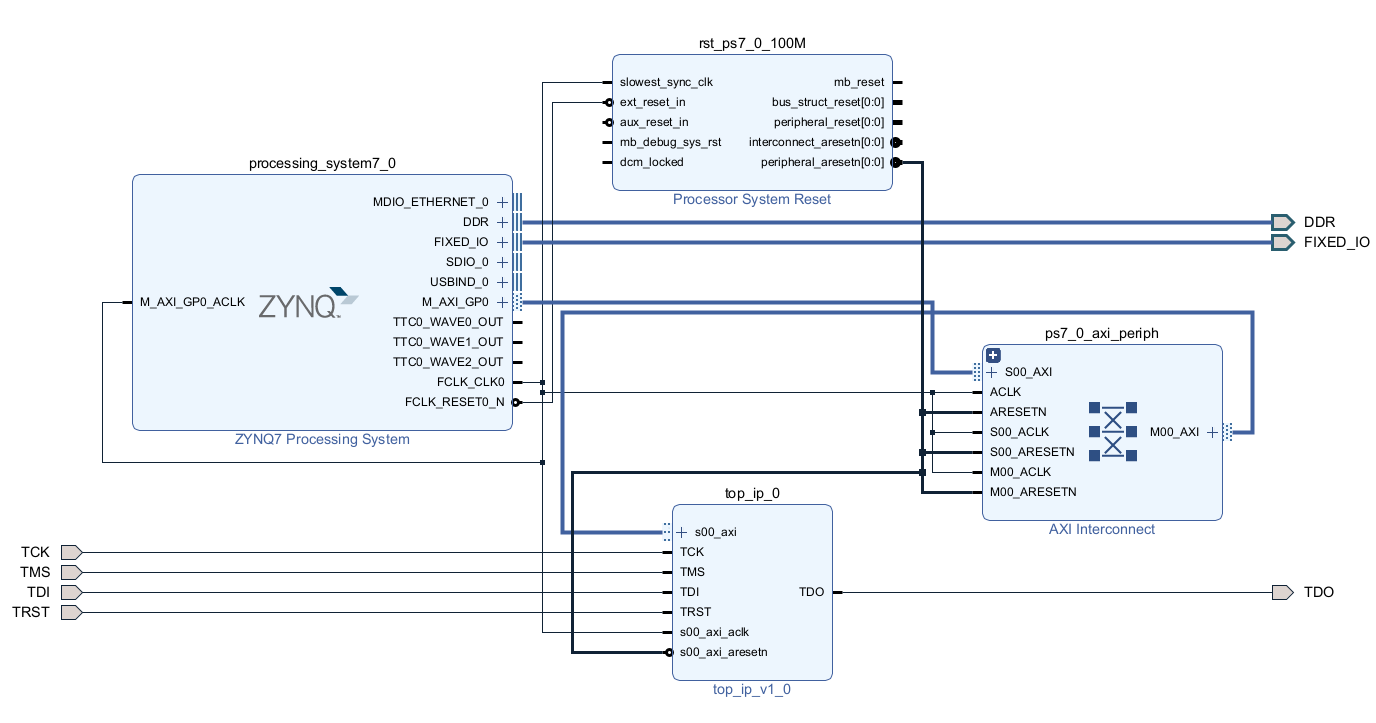
\includegraphics[width=1\linewidth]{Image/BD1.png}
    \caption{SoC Block diagram}
    \label{fig:enter-label}
\end{figure}


\vspace{6mm}
AXI interconnect block plays a crucial role in facilitating communication and data transfer between different AXI masters and slaves. In this case, the AXI master is a processor that initiates data transfer with the custom IP which is an AXI slave. The interconnect block performs address decoding to route transactions from masters to the appropriate slaves based on the address information in the AXI transactions. The AXI interconnect may include an arbitration mechanism to resolve contention for the bus when multiple masters are trying to access the same slave simultaneously. In this custom SoC the AXI interconnect block is configured to have one master and one slave.

\newpage
AXI interconnect signal description:
\begin{table}[H]
		%\begin{table}[ht]
		\centering
		\begin{tabularx}{\textwidth}{|p{3cm}  |p{2cm} |X|}
			\hline
			S00\_AXI & INPUT & Master Interfacing with Slave \\
			\hline
			M00\_AXI & OUTPUT & Slave Interfacing with Master   \\
            \hline
			ACLK & INPUT & Clock to AXI Interconnect \\
			\hline
			ARESETN & INPUT & Reset Signal to AXI Interconnect \\
			\hline
			S00\_ACLK & INPUT & Clock to AXI Slave \\
			\hline
            S00\_ARESETN & INPUT & Reset Signal to AXI Slave \\
			\hline
            M00\_ACLK & INPUT & Clock to AXI Master \\
			\hline
            M00\_ARESETN & INPUT & Reset Signal to Master \\
			\hline
		\end{tabularx}
		\caption{AXI Interconnect}
		%\label{tab:01Glossary Type Descriptions}
	\end{table}

\vspace{6mm}
Custom IP signal description:
 \begin{table}[H]
		%\begin{table}[ht]
		\centering
		\begin{tabularx}{\textwidth}{|p{3cm}  |p{3cm} |X|}
			\hline
			TCK & INPUT &  Clock signal to control Test Access Port\\
			\hline
			TMS & INPUT & Signal which decides shiting of Data in and out through data/Instruction register   \\
            \hline
			TDI & INPUT & To serially inputting test data\\
			\hline
               TDO & OUTPUT & To serially outputting test data\\
			\hline
			TRST & INPUT &  To reset the tets logic\\
			\hline
			s00\_axi\_aclk & INPUT & clock input for a specific AXI interface\\
			\hline
            s00\_axi\_aresetn & INPUT &  reset signal for a specific AXI interface\\
			\hline
		\end{tabularx}
		\caption{Custom IP}
		%\label{tab:01Glossary Type Descriptions}
	\end{table}
\subsection{Custom IP Hierarchy}

The provided diagram illustrates the structure of the customized IP. It is evident from the diagram that the Register File and Scan Chain modules are instantiated within the AXI environment. Consequently, all ports of the register file are associated with AXI registers, establishing a memory-mapped connection with the ARM core. This configuration enables the seamless transfer of data from the ARM core into the register file by utilizing designated memory locations.

\begin{figure}[h]
    \centering
    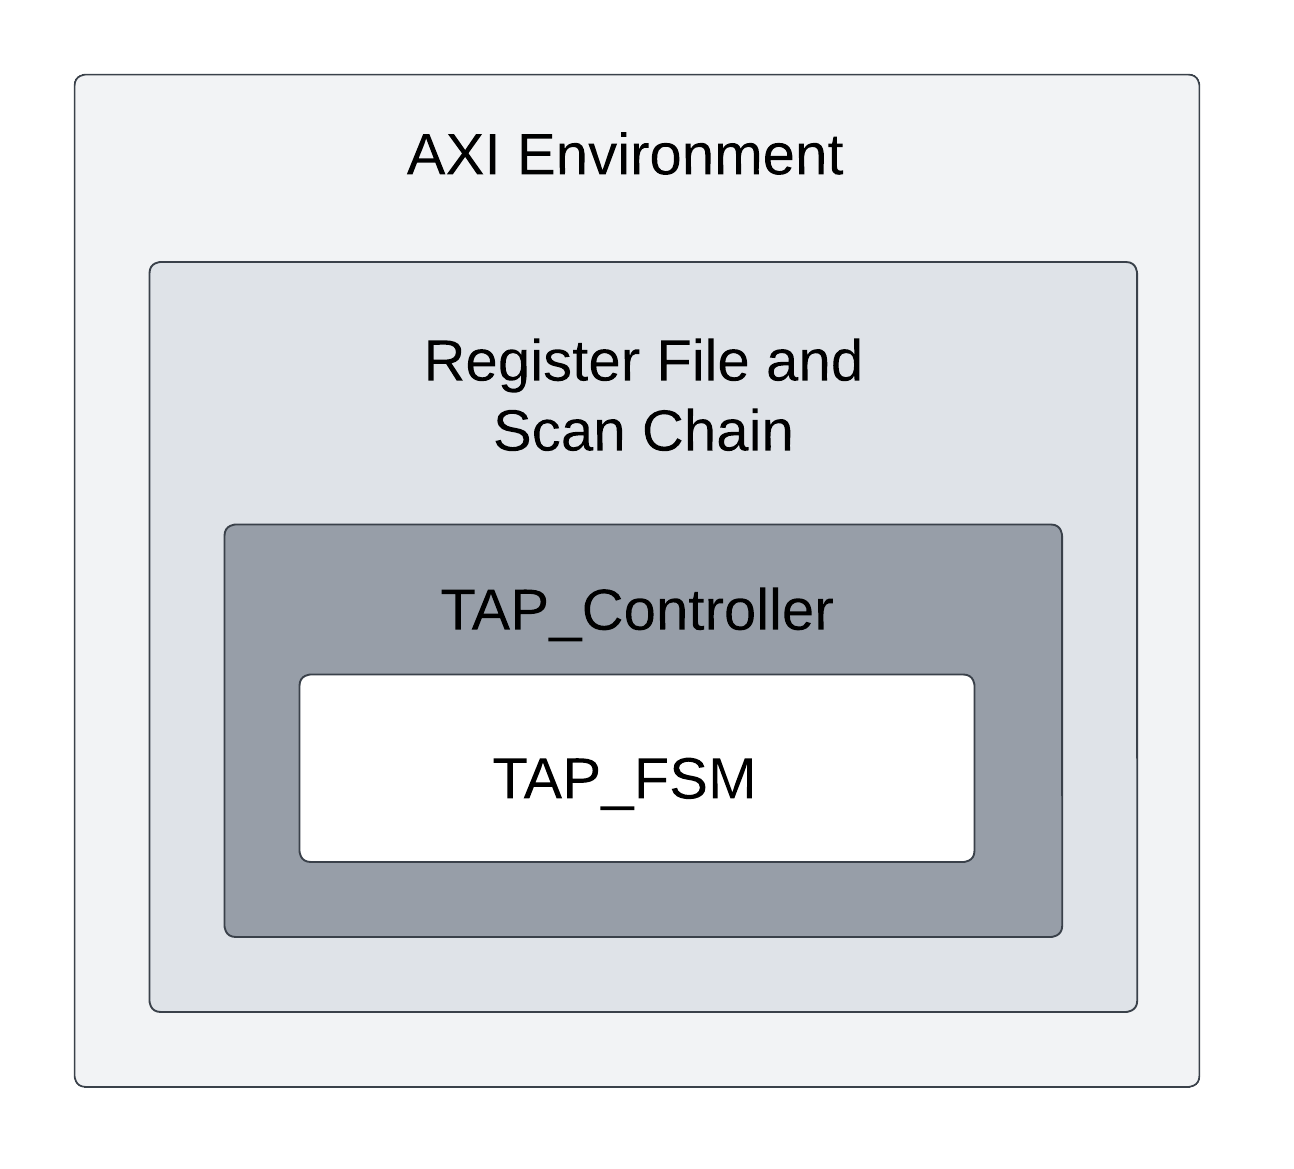
\includegraphics[width=0.5\linewidth]{Image/Heirarachy.png}
    \caption{Custom IP}
    \label{fig:enter-label}
\end{figure}

\vspace{2mm}

Certain ports of the TAP controller, including TDI, TDO, TMS, TCK, and TRST, are not linked to the AXI registers. These ports are essential for receiving data from a JTAG network and are exposed at the top level of the files, serving as IO ports for the custom IP. The data received through these IO ports from the JTAG network is then directed to the TAP controller within the design. 



 



\section{Custom IP simulation}

To validate the functionality of the custom IP and incorporate any required modifications prior to the physical construction of the system, we employed VHDL simulation. VHDL simulation is the practice of utilizing a software tool to simulate and assess the performance of a digital circuit based on VHDL language descriptions. In this process, the simulation tool interprets the VHDL code, particularly the testbench component that outlines the expected behaviour of the circuit, and produces a simulated model of the circuit. Subsequently, we examined the simulation outcomes using waveform viewers available in the Vivado platform.
\subsection{Test case 1}
Test the functionality of the register file.

\begin{itemize}
    \item Write Operation:


\textbf{Input: }write x”ffffffff”, x"0f0f0f0f" and x"0000ffff" data into the registers R31, R30 and R29 respectively when regwr signal is LOW.

\textbf{Expected output: }Storing the above-mentioned data into the registers R31, R30 and R29 of the register file.
\end{itemize}
\vspace{2mm}

\begin{figure}[h]
    \centering
    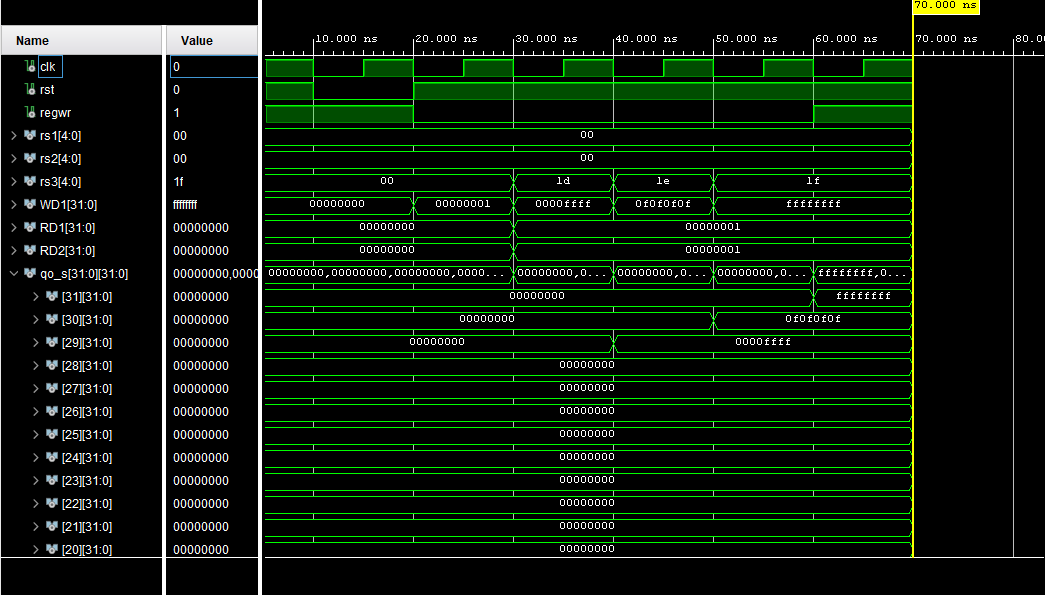
\includegraphics[width=0.8\linewidth]{Image/WO2.png}
    \caption{Write Operation}
    \label{fig:enter-label}
\end{figure}
\vspace{2mm}

\textbf{Observations:} From the above simulation output figure 9.2, it can be observed that the rs3 signal holds the address of the registers R29, R30 and R31 and it can be seen that during the falling edge of every clock cycle data present in the WD3 register is being written into respective registers of register file qo\_s.
\newpage
\begin{itemize}
    \item Read Operation:

\textbf{Input:} Read the data present in the registers R31 and R30 of the register file into the internal registers WD1 and WD2.

\textbf{Expected output:} To fetch the data present in R31 and R30 registers of the register file and then store it into the WD1 and WD2 registers respectively.
\end{itemize}

 \begin{figure}[h]
    \centering
    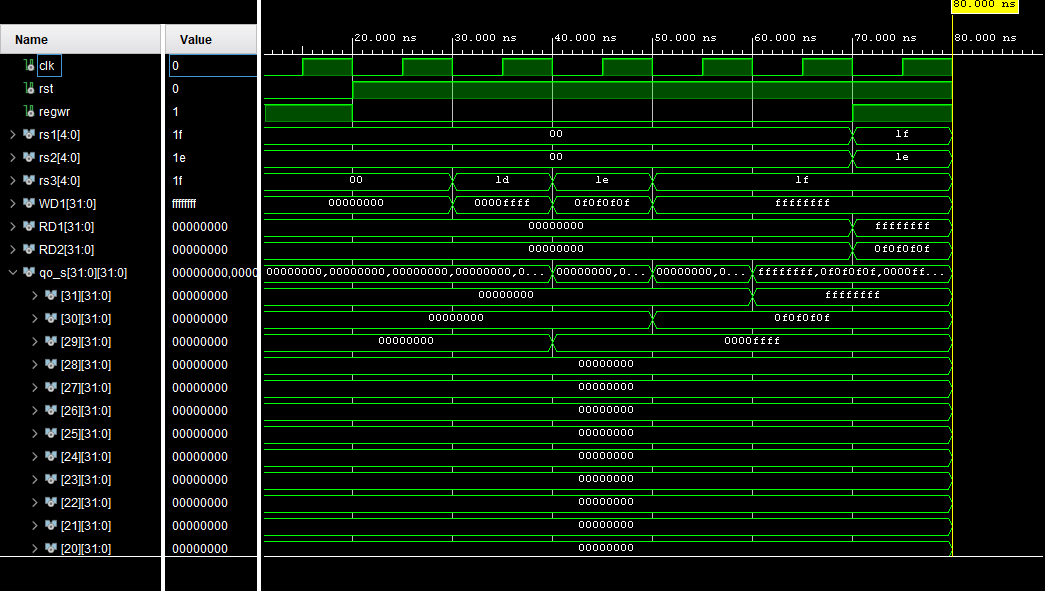
\includegraphics[width=0.8\linewidth]{Image/RO2.png}
    \caption{Read Operation}
    \label{fig:enter-label}
\end{figure}
%\pagebreak
%\newpage
\subsection{Test case 2}

Test the functionality of the scan chain.
\vspace{2mm}

\textbf{Scan chain:}
\vspace{2mm}

From the below simulation figure 9.4, it can be observed that at the simulation period 240ns the current state of the TAP controller is Shift\_DR and scan functionality is enabled as scan\_enable signal is HIGH. The Instruction register ir2\_s has a value of 2, this implies that the TAP controller is currently in scan chain mode. Also, it can be observed that the scan\_in\_signal is also made high for one clock cycle. The states of the above-mentioned signals enable the TAP controller and register file to be in scan mode.

\newpage

\begin{figure}[h]
    \centering
    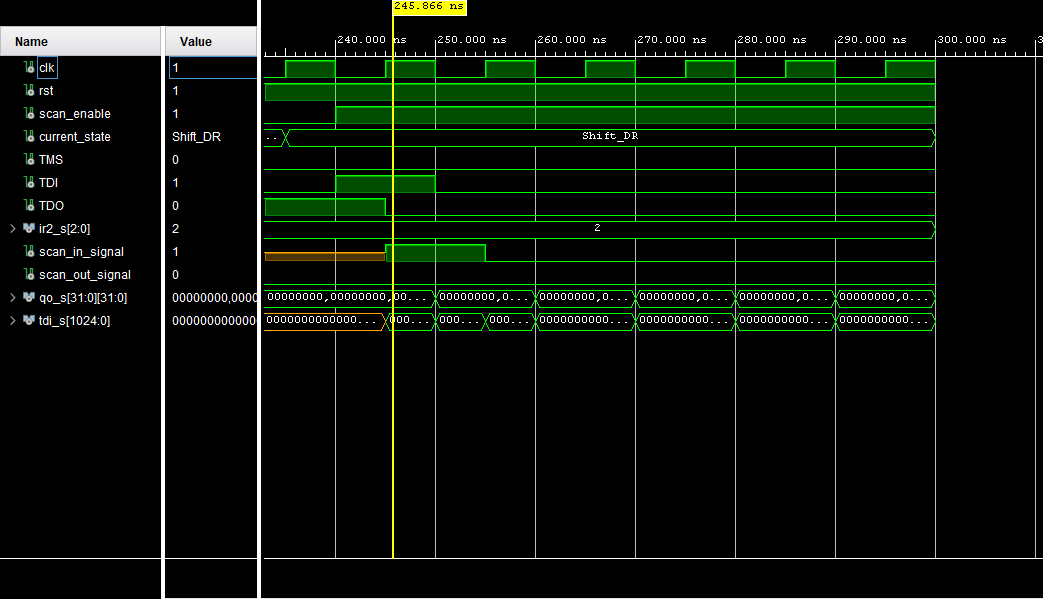
\includegraphics[width=0.8\linewidth]{Image/WO3.png}
    \caption{Scan chain 1}
    \label{Scan chain 1}
\end{figure}

 Scan\_in\_data signal will now be shifted from 1st scan flipflop to the 1024th scan flipflop after 1023 clock cycles and will eventually reflect in the scan\_out\_data signal and will pass through TDO port of the TAP controller. This can be observered in the below figure 8.5.


\begin{figure}[h]
    \centering
    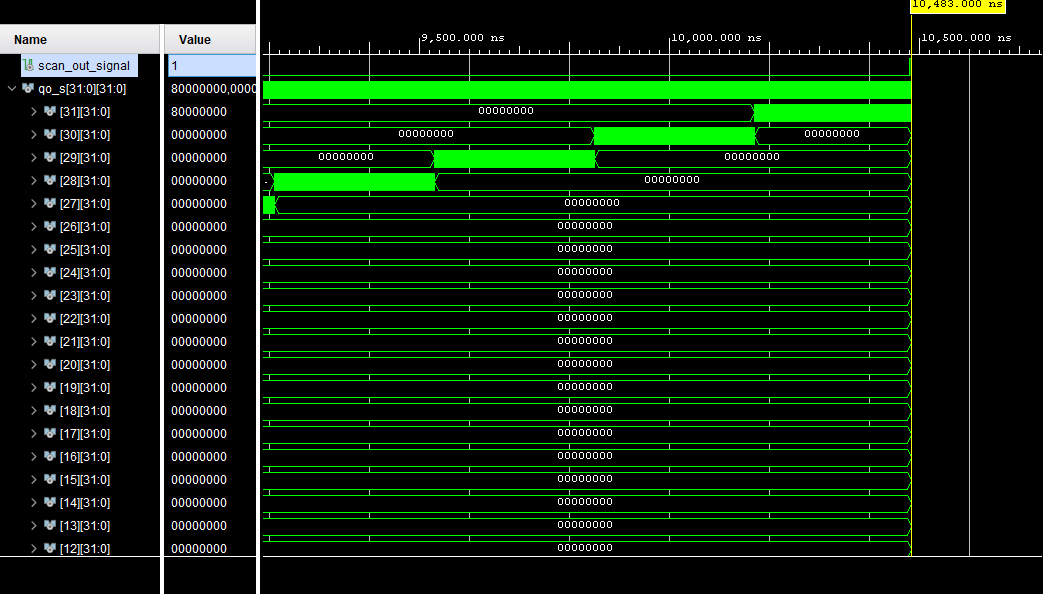
\includegraphics[width=0.8\linewidth]{Image/RO3.png}
    \caption{Scan chain 2}
    \label{Scan chain 2}
\end{figure}
\pagebreak
\vspace{2mm}

\subsection{Test case 3}
Test the functionality of the Bypass.
\vspace{2mm}

\textbf{Bypass:}
\vspace{2mm}

In the Bypass scenario, test data is directly passed to the output as data from TDI(Input) passed to TDO(Output) on rising edge in ShiftDR state.

\begin{figure}[h]
    \centering
    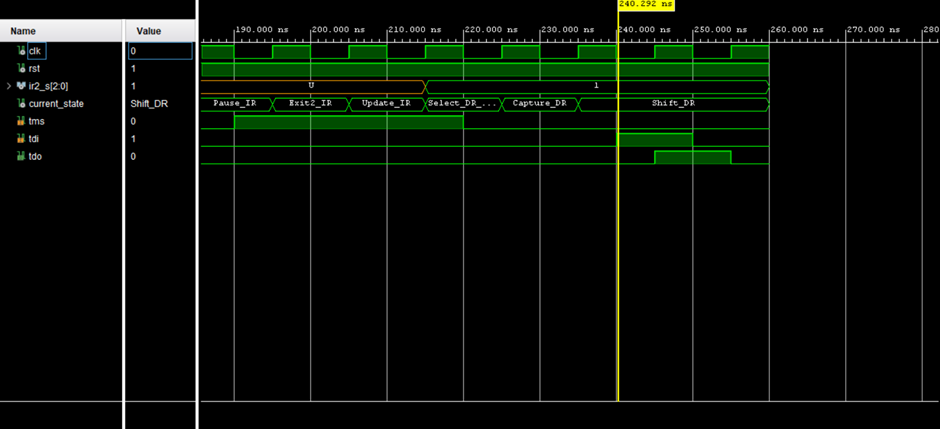
\includegraphics[width=0.8\linewidth]{Image/Bypass.png}
    \caption{Bypass}
    \label{fig:Bypass}
\end{figure}

\section{Synthesis}

The synthesis process entails examining the design, optimizing logic, and translating a high-level hardware description, written in a hardware description language like VHDL, into a lower-level representation, typically in the form of a gate-level netlist. This gate-level netlist, generated as output, serves as input for the subsequent place-and-route implementation of the design on either an FPGA or ASIC.
\vspace{2mm}
Upon completion of the block design, a HDL Wrapper is generated in the Vivado platform, automating the VHDL code generation for the entire block design. In the final step of the Vivado design process, a Bitstream, along with a constraint file, can be produced and downloaded into the target board.

\section{ Application development}

After the hardware synthesis process has been completed, the focus shifts to developing the software application that will run on the synthesized hardware. Vitis platform is a collection of hardware and software components. After synthesis, we need to create a platform that includes the synthesized hardware design along with the necessary software components. HDL wrapper XSA file is imported into the Vitis IDE for further BSP (Board support packages) generation for the custom hardware.
\vspace{2mm}

For our custom IP which includes a register file, we have written some basic drivers which will enable application development for the custom hardware.
\newpage
\begin{table}[h]
		%\begin{table}[ht]
		\centering
		\begin{tabularx}{\textwidth}{|p{3cm}   |X|}
			\hline
			\textbf{Driver}  & \textbf{Description}\\
			\hline
			initRegFile & Initialize base address depending on the memory mapping of custom IP     \\
            \hline
			writeRegFile & Writes data into the desired register of the register file  \\
			\hline
			readRegFileR1 & Reads data from the RD1 of the register file    \\
			\hline
			readRegFileR2 & Reads data from the RD2 of the register file    \\
			\hline
            resetRegFile & Reset signal for the register file   \\
			\hline
            writeDisable & To disable the write signal in the register file   \\
			\hline
           scanEnable & To enable scan chain functionality of the register file  \\
			\hline
		\end{tabularx}
		\caption{Basic Drivers}
		%\label{tab:01Glossary Type Descriptions}
	\end{table}
